% Provenance (never printed): see sources/outline_sources.md (Year 2: partial melting of the
% mantle; solidus and geotherm; decompression, hydration and heating; degree of melting;
% binary and ternary phase diagrams applied to rocks).
% Curves from figdata/bachelor-2/melting.py (Bowen 1915 diopside-anorthite, Bowen and
% Andersen 1914 forsterite-silica, Katz et al. 2003 melting of peridotite); exercise and
% problem values in the Book 4 scratch calculator calc/ch07.py.
\chapter{A fusão do manto}\label{ch:b2:mantle-melting}

O manto é sólido. As ondas sísmicas de cisalhamento o atravessam de cima a baixo, e o
\omterm{def:b2:mantle-melting:peridotites}{peridotito} trazido dele é uma rocha cristalina. No entanto, só ao longo das dorsais oceânicas
ele fornece uns vinte quilômetros cúbicos de crosta oceânica nova por ano,
cada metro cúbico dela feito a partir de um fundido. O paradoxo se desfaz quando se sabe
que o manto não funde porque é aquecido: ele funde porque a
pressão sobre ele cai, ou porque se lhe acrescenta água. Sob uma dorsal, o
manto sobe, sua pressão cai mais depressa que sua temperatura, e ele cruza sua
curva de fusão; acima de uma placa que afunda, a água liberada pela placa rebaixa essa
curva sob a cunha mantélica. Nos dois casos, só uma pequena fração da rocha
funde, e essa fração, separada de seu resíduo, torna-se o basalto do
fundo oceânico e dos arcos vulcânicos. Este capítulo descreve primeiro a rocha do
manto e os diagramas de fase que dizem como tais rochas fundem, e depois acompanha o
manto em sua subida sob uma dorsal até a espessura da crosta que ele produz.
% ledger: white:crust (Book 3), data:pb2002 (Book 3), katz03:solidus

\begin{recall}
\textbf{Do volume do segundo ano dos livros de química}: os diagramas de fase binários, o
solidus e o liquidus, o ponto eutético, a fusão congruente, as soluções sólidas
e a regra da alavanca, pela qual as proporções de duas fases coexistentes são
inversamente proporcionais às suas distâncias à composição global.
\textbf{Dos livros de física}: o calor específico, o calor latente, a entropia
e o segundo princípio, pelo qual um processo adiabático reversível conserva a entropia.
\textbf{Do volume do primeiro ano}: os principais minerais formadores de rochas, olivina,
piroxênios, granada e espinélio, suas soluções sólidas e o número de Mg; a
adiabática do manto, $\mathrm dT/\mathrm dz = \alpha gT/c_p$; a crosta oceânica,
com \qty[uncertainty-mode=separate]{7.1 \pm 0.8}{km} de espessura longe dos pontos quentes e
cerca de \qty{20}{km} sobre o centro de uma pluma; as placas em subducção e a água que elas
carregam. \textbf{Do \cref{ch:b2:elements-in-the-earth}}: o \omterm{def:b2:elements-in-the-earth:morb-oib}{basalto de dorsal meso-oceânica}
(MORB), os coeficientes de partição e os \omterm{def:b2:elements-in-the-earth:partition}{elementos incompatíveis}.
\end{recall}

\section{A rocha do manto}\label{sec:b2:mantle-melting:rock}

A rocha do manto chega à superfície como fragmentos trazidos por \omterm{def:b2:magma-emplacement:magma}{magmas}, os
xenólitos, e como a base de lascas de litosfera oceânica empurradas sobre os
continentes, os ofiolitos. Quase toda ela é \omterm{def:b2:mantle-melting:peridotites}{peridotito}.
% ledger: geo:peridotite (Book 2), tulane:ocean-basins (Book 2)

\begin{definition}[O peridotito e seus tipos]\label{def:b2:mantle-melting:peridotites}
Um \emph{peridotito}\index{peridotito} é uma rocha ultramáfica de granulação grossa
que contém mais de \qty{40}{\percent} de olivina, sendo o resto piroxênios e um
pouco de um mineral aluminoso (espinélio ou granada). Um
\emph{dunito}\index{dunito} contém mais de \qty{90}{\percent} de olivina. Abaixo
disso, um \emph{lherzolito}\index{lherzolito} contém ortopiroxênio e
clinopiroxênio; um \emph{harzburgito}\index{harzburgito} contém ortopiroxênio, mas
quase nenhum clinopiroxênio; um wehrlito contém clinopiroxênio, mas quase nenhum
ortopiroxênio. As rochas com menos de \qty{40}{\percent} de olivina são piroxenitos.
\end{definition}
% ledger: bgs:ultramafic

A classificação é lida em um triângulo cujos vértices são a olivina, o
ortopiroxênio e o clinopiroxênio (a figura abaixo): cada ponto representa uma rocha,
e suas distâncias aos três lados dão as proporções dos três
minerais. Uma composição modelo do manto superior empobrecido que funde sob
as dorsais tem \qty{57}{\percent} de olivina,
\qty{28}{\percent} de ortopiroxênio, \qty{13}{\percent} de clinopiroxênio e
\qty{2}{\percent} de espinélio: um \omterm{def:b2:mantle-melting:peridotites}{lherzolito}.
% ledger: liang21:dmm-mode

\begin{omfigure}
\centering
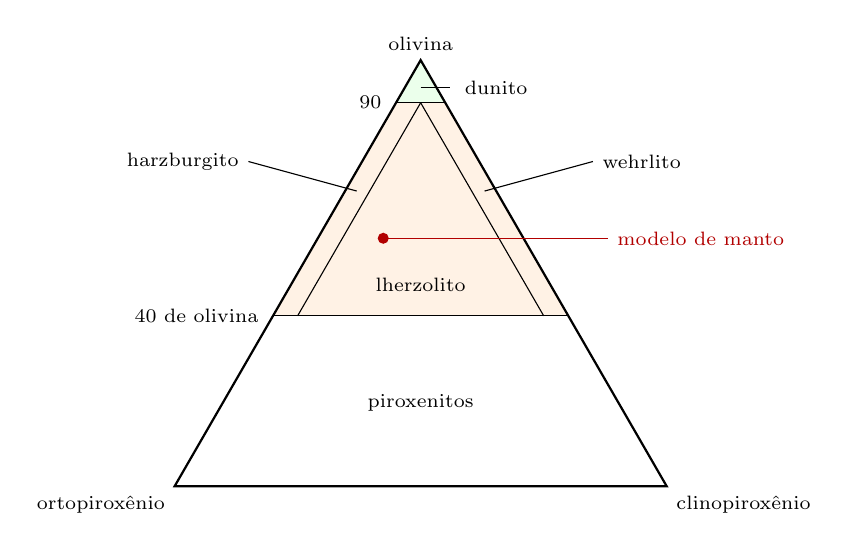
\begin{tikzpicture}[x=1.25cm, y=1.25cm, font=\scriptsize]
\coordinate (O) at (2.5,4.330); \coordinate (P) at (0,0); \coordinate (C) at (5,0);
\fill[green!8] (2.25,3.897) -- (2.75,3.897) -- (O) -- cycle;
\fill[orange!10] (1,1.732) -- (2.25,3.897) -- (2.75,3.897) -- (4,1.732) -- cycle;
\draw[thick] (O) -- (P) -- (C) -- cycle;
\draw (2.25,3.897) -- (2.75,3.897);
\draw (1,1.732) -- (4,1.732);
\draw (2.5,3.897) -- (1.25,1.732);
\draw (2.5,3.897) -- (3.75,1.732);
\node[anchor=south] at (O) {olivina};
\node[anchor=north east] at (P) {ortopiroxênio};
\node[anchor=north west] at (C) {clinopiroxênio};
\node[anchor=west] at (2.85,4.05) {dunito};
\draw (2.5,4.05) -- (2.8,4.05);
\node at (2.5,2.05) {lherzolito};
\draw (1.85,3.0) -- (0.75,3.3) node[anchor=east] {harzburgito};
\draw (3.15,3.0) -- (4.25,3.3) node[anchor=west] {wehrlito};
\node at (2.5,0.85) {piroxenitos};
\node[anchor=east] at (0.95,1.732) {\qty{40}{\percent} de olivina};
\node[anchor=east] at (2.2,3.897) {\qty{90}{\percent}};
\fill[red!70!black] (2.12,2.52) circle (2pt);
\draw[red!70!black] (2.12,2.52) -- (4.4,2.52) node[anchor=west] {modelo de manto};
\end{tikzpicture}
\par\smallskip{\small Classificação dos \omterm{def:b2:mantle-melting:peridotites}{peridotitos} e dos piroxenitos por suas
proporções de olivina, ortopiroxênio e clinopiroxênio (segundo o esquema do British
Geological Survey). As faixas estreitas ao longo dos dois lados superiores contêm as
rochas quase sem clinopiroxênio (\omterm{def:b2:mantle-melting:peridotites}{harzburgito}) ou sem ortopiroxênio (wehrlito).
O ponto vermelho é o manto superior modelo sob as dorsais (57, 28 e
\qty{13}{\percent}, renormalizados sem seus \qty{2}{\percent} de espinélio).}
\end{omfigure}
% ledger: bgs:ultramafic, liang21:dmm-mode

Os três \omterm{def:b2:mantle-melting:peridotites}{peridotitos} não são três tipos de rocha independentes: são etapas de
um mesmo processo. O clinopiroxênio e o mineral aluminoso se esgotam primeiro quando o
\omterm{def:b2:mantle-melting:peridotites}{peridotito} funde (\cref{sec:b2:mantle-melting:decompression}), de modo que um \omterm{def:b2:mantle-melting:peridotites}{lherzolito}
que perdeu um fundido fica mais pobre neles; após fusão suficiente, ele é um
\omterm{def:b2:mantle-melting:peridotites}{harzburgito}, e uma rocha que perdeu quase todo o seu piroxênio é um \omterm{def:b2:mantle-melting:peridotites}{dunito}.
% ledger: katz03:melting

\begin{definition}[Manto fértil e manto residual]\label{def:b2:mantle-melting:fertility}
Um \emph{manto fértil}\index{manto fértil} é um \omterm{def:b2:mantle-melting:peridotites}{peridotito}, tipicamente um
\omterm{def:b2:mantle-melting:peridotites}{lherzolito}, que ainda contém o clinopiroxênio e o mineral aluminoso a partir dos
quais se faz o basalto. Um \emph{manto residual}\index{manto residual} é o
\omterm{def:b2:mantle-melting:peridotites}{peridotito} deixado para trás depois que um fundido foi extraído dele: mais pobre em
clinopiroxênio, alumínio, cálcio e \omterm{def:b2:elements-in-the-earth:partition}{elementos incompatíveis}, mais rico em
olivina e com um número de Mg mais alto.
\end{definition}

O \omterm{def:b2:isotope-geochemistry:reservoirs}{manto empobrecido} isotópico do \cref{ch:b2:isotope-geochemistry} é um reservatório,
definido por suas razões; um \omterm{def:b2:mantle-melting:fertility}{manto residual} é uma rocha, definida pelo que perdeu.
Os dois estão ligados, já que o \omterm{def:b2:isotope-geochemistry:reservoirs}{manto empobrecido} é empobrecido porque um fundido foi
extraído dele há muito tempo, mas um se lê em um espectrômetro de massa e o outro
ao microscópio.

\section{Diagramas de fase das rochas}\label{sec:b2:mantle-melting:diagrams}

Uma rocha é uma mistura de minerais, e ela funde em um intervalo de temperaturas, não em
um ponto. Os diagramas que descrevem isso foram medidos primeiro em misturas de
minerais sintéticos puros, mantendo uma pequena carga a uma temperatura conhecida até que ela
atingisse o equilíbrio, temperando-a e procurando ao microscópio o vidro,
que era líquido, e os cristais.

\subsection*{Um eutético binário: diopsídio e anortita}

Um basalto é formado essencialmente de um plagioclásio cálcico e de um clinopiroxênio, e
Bowen escolheu a anortita e o diopsídio puros como seu modelo mais simples. Misturados e aquecidos,
eles formam um sistema eutético
comum (a figura abaixo): o diopsídio funde a \qty{1391.5}{\celsius} e a anortita
a \qty{1550}{\celsius}, mas uma mistura de \qty{58}{\percent} de diopsídio e
\qty{42}{\percent} de anortita em massa funde completamente a \qty{1270}{\celsius}.
% ledger: bowen15:di-an

\begin{omfigure}
\centering
\begin{tikzpicture}
\begin{axis}[omrecord, width=0.78\linewidth, height=6cm,
  xmin=0, xmax=100, ymin=1200, ymax=1600,
  xlabel={anortita (\unit{\percent} em massa)}, ylabel={temperatura (\unit{\celsius})},
  y tick label style={/pgf/number format/1000 sep={}},
  tick label style={font=\scriptsize}, label style={font=\small}]
\addplot[very thick, black] table[x=x_an, y=T] {figdata/out/bachelor-2-melting-di-an-liq.dat};
\addplot[only marks, mark=*, mark size=1.6pt, blue!70!black] table[x=x_an, y=T] {figdata/out/bachelor-2-melting-di-an-data.dat};
\draw[thick] (axis cs:0,1270) -- (axis cs:100,1270);
\draw[densely dotted, red!70!black, thick] (axis cs:20,1590) -- (axis cs:20,1270);
\draw[->, red!70!black, thick] (axis cs:20,1350) -- (axis cs:41,1272);
\fill[red!70!black] (axis cs:20,1350) circle (1.6pt);
\node[font=\scriptsize] at (axis cs:55,1500) {líquido};
\node[font=\scriptsize, align=center] at (axis cs:10,1300) {diopsídio\\+ líquido};
\node[font=\scriptsize, align=center] at (axis cs:72,1360) {anortita + líquido};
\node[font=\scriptsize] at (axis cs:68,1235) {diopsídio + anortita};
\node[font=\scriptsize, anchor=north east] at (axis cs:41,1267) {E, \qty{1270}{\celsius}};
\node[font=\scriptsize, anchor=west, red!70!black] at (axis cs:21,1360) {primeiro diopsídio};
\end{axis}
\end{tikzpicture}
\par\smallskip{\small O sistema diopsídio--anortita à pressão atmosférica, segundo
os experimentos de têmpera de Bowen (1915): temperaturas do liquidus (pontos, médias dos
intervalos de têmpera) e o eutético E. Em vermelho, o resfriamento de um líquido com
\qty{20}{\percent} de anortita: o diopsídio cristaliza a partir de \qty{1350}{\celsius}, o
líquido desce pelo liquidus até E, e o resto cristaliza ali como uma mistura dos
dois minerais.}
\end{omfigure}
% ledger: bowen15:di-an

Lido de cima, o diagrama dá a ordem de cristalização. Um líquido com
\qty{20}{\percent} de anortita começa a cristalizar diopsídio a
\qty{1350}{\celsius}; o líquido, perdendo diopsídio, enriquece-se em anortita e
desce pelo liquidus até atingir o eutético, onde a anortita se junta ao
diopsídio e a temperatura permanece em \qty{1270}{\celsius} até que todo o líquido tenha
desaparecido. Lido de baixo, ele diz como a rocha funde: quaisquer que sejam as proporções dos
dois minerais, o primeiro líquido aparece a \qty{1270}{\celsius} e tem a
composição eutética. Essa é a primeira lição para o manto. O primeiro fundido de uma
rocha não tem a composição da rocha: tem a composição fixada pelos
minerais a partir dos quais funde, e aparece a uma temperatura bem abaixo dos pontos de
fusão de todos eles.

\subsection*{Fusão incongruente: forsterita e sílica}

Certos minerais não fundem em um líquido de sua própria composição.

\begin{definition}[Fusão incongruente, ponto peritético]\label{def:b2:mantle-melting:peritectic}
Um mineral apresenta \emph{fusão incongruente}\index{fusão incongruente} quando, ao ser
aquecido, se decompõe em outro sólido e em um líquido de composição diferente,
em vez de fundir em um líquido de sua própria composição. Em um diagrama de fase
binário, o ponto em que esse líquido coexiste com os dois sólidos é um
\emph{ponto peritético}\index{ponto peritético}: ao contrário de um eutético, ele não fica
entre as composições dos dois sólidos.
\end{definition}

A enstatita, o ortopiroxênio magnesiano \ce{MgSiO3}, funde de modo incongruente. À
pressão atmosférica, ela se decompõe a \qty{1557}{\celsius} em forsterita,
\ce{Mg2SiO4}, e em um líquido ligeiramente mais rico em sílica que ela; só a
\qty{1577}{\celsius} toda a forsterita se dissolveu (a figura abaixo). Bowen
e Andersen verificaram em 1914 que a decomposição dá \qty{5.5}{\percent} de
forsterita e \qty{94.5}{\percent} de líquido, como a regra da alavanca prevê a partir
das três composições (\cref{exo:b2:mantle-melting:6}). Mais para o lado da sílica, a enstatita e a
cristobalita fundem juntas em um eutético, a \qty{1543}{\celsius}.
% ledger: bowen14:mgo-sio2

\begin{omfigure}
\centering
\begin{tikzpicture}
\begin{axis}[omrecord, width=0.78\linewidth, height=6cm,
  xmin=40, xmax=66, ymin=1450, ymax=1950,
  xlabel={\ce{SiO2} (\unit{\percent} em massa)}, ylabel={temperatura (\unit{\celsius})},
  y tick label style={/pgf/number format/1000 sep={}},
  tick label style={font=\scriptsize}, label style={font=\small}]
\addplot[very thick, black] table[x=x_sio2, y=T] {figdata/out/bachelor-2-melting-fo-sio2-liq.dat};
\addplot[very thick, black, dashed] table[x=x_sio2, y=T] {figdata/out/bachelor-2-melting-fo-sio2-fo.dat};
\draw[thick] (axis cs:42.71,1450) -- (axis cs:42.71,1890);
\draw[thick] (axis cs:42.71,1557) -- (axis cs:60.86,1557);
\draw[thick] (axis cs:59.85,1450) -- (axis cs:59.85,1557);
\draw[thick] (axis cs:59.85,1543) -- (axis cs:66,1543);
\fill (axis cs:60.86,1557) circle (1.6pt);
\fill (axis cs:64.87,1543) circle (1.6pt);
\fill (axis cs:42.71,1890) circle (1.6pt);
\node[font=\scriptsize, anchor=south west] at (axis cs:42.9,1890) {a forsterita funde, \qty{1890}{\celsius}};
\node[font=\scriptsize] at (axis cs:56,1800) {líquido};
\node[font=\scriptsize] at (axis cs:48,1680) {forsterita + líquido};
\node[font=\scriptsize] at (axis cs:51,1500) {forsterita + enstatita};
\node[font=\scriptsize, align=center] at (axis cs:63,1495) {enstatita +\\cristobalita};
\node[font=\scriptsize, anchor=south] at (axis cs:61.3,1560) {P};
\node[font=\scriptsize, anchor=south] at (axis cs:64.87,1546) {E};
\node[font=\scriptsize, anchor=north, rotate=90] at (axis cs:42.71,1650) {\ce{Mg2SiO4}};
\node[font=\scriptsize, anchor=south, rotate=90] at (axis cs:59.85,1510) {\ce{MgSiO3}};
\end{axis}
\end{tikzpicture}
\par\smallskip{\small Parte do sistema \ce{MgO}--\ce{SiO2} à pressão
atmosférica, segundo Bowen e Andersen (1914). A enstatita (\ce{MgSiO3}) funde de modo
incongruente no peritético P, a \qty{1557}{\celsius}, em forsterita e em um
líquido com \qty{60.9}{\percent} de \ce{SiO2}; E é o eutético enstatita--cristobalita,
a \qty{1543}{\celsius}. O liquidus da forsterita só foi medido perto da
enstatita: a parte tracejada é traçada em linha reta até o ponto de fusão da forsterita.}
\end{omfigure}
% ledger: bowen14:mgo-sio2

O peritético é a segunda lição para o manto. Quando um \omterm{def:b2:mantle-melting:peridotites}{peridotito} funde, seu
ortopiroxênio não se dissolve simplesmente: ele cede olivina ao resíduo e sílica
ao fundido. O fundido é portanto mais rico em sílica que os piroxênios, e o
resíduo mais rico em olivina que a rocha: o caminho do \omterm{def:b2:mantle-melting:peridotites}{lherzolito} ao \omterm{def:b2:mantle-melting:peridotites}{harzburgito}
e ao \omterm{def:b2:mantle-melting:peridotites}{dunito}.

\subsection*{Três componentes: o diagrama ternário}

As rochas reais têm mais de dois minerais. Com três, a composição exige um
triângulo, e a temperatura torna-se uma terceira dimensão.

\begin{definition}[Diagrama de fase ternário, linha cotética, eutético ternário]\label{def:b2:mantle-melting:ternary}
Um \emph{diagrama de fase ternário}\index{diagrama de fase ternário} representa os
equilíbrios de um sistema de três componentes a uma pressão dada: cada ponto de um
triângulo representa uma composição, os vértices os componentes puros, e a
superfície do liquidus é traçada como curvas de nível de temperatura ou como os campos dos
minerais que cristalizam primeiro. Uma \emph{linha cotética}\index{linha cotética} é
a linha ao longo da qual o líquido está saturado em dois minerais ao mesmo tempo e
cristaliza ambos ao se resfriar. As linhas cotéticas descem a partir dos eutéticos
binários situados nos lados do triângulo e se encontram no \emph{eutético
ternário}\index{eutético ternário}, a temperatura mais baixa na qual existe líquido,
onde os três minerais cristalizam juntos.
\end{definition}

\begin{method}[Ler um caminho de cristalização em um diagrama ternário]\label{met:b2:mantle-melting:ternary}
Localize-se a composição global $X$ no triângulo e o campo em que ela se encontra:
o mineral desse campo cristaliza primeiro. Enquanto esse mineral cristaliza sozinho,
o líquido se desloca em linha reta afastando-se diretamente do vértice do mineral,
passando por $X$, porque retirar um componente puro só altera sua proporção; pela
regra da alavanca, a fração em massa de cristais é a distância de $X$ ao líquido
dividida pela distância do vértice ao líquido. Quando o líquido atinge uma
\omterm{def:b2:mantle-melting:ternary}{linha cotética}, o segundo mineral se junta a ele e o líquido segue a cotética
descendo até o \omterm{def:b2:mantle-melting:ternary}{eutético ternário}, onde o último líquido cristaliza. Um componente
que não entra em nenhum dos cristais permanece no líquido, de modo que sua concentração dá
a fração de líquido restante: $f_{\text{líquido}} = c_X/c_{\text{líquido}}$.
\end{method}

\begin{omfigure}
\centering
\begin{tikzpicture}[x=1cm, y=1cm, font=\scriptsize]
\coordinate (A) at (3,5.196); \coordinate (B) at (0,0); \coordinate (C) at (6,0);
\coordinate (eAB) at (1.2,2.078); \coordinate (eAC) at (4.65,2.338);
\coordinate (eBC) at (3.9,0); \coordinate (E) at (3.45,1.299);
\coordinate (X) at (3.0,3.118); \coordinate (L) at (3.0,1.455);
\fill[green!8] (A) -- (eAB) -- (E) -- (eAC) -- cycle;
\fill[orange!10] (B) -- (eAB) -- (E) -- (eBC) -- cycle;
\fill[blue!7] (C) -- (eAC) -- (E) -- (eBC) -- cycle;
\draw[thick] (A) -- (B) -- (C) -- cycle;
\draw[very thick, -{Stealth[length=4pt]}] (eAB) -- ($(eAB)!0.55!(E)$);
\draw[very thick] ($(eAB)!0.5!(E)$) -- (E);
\draw[very thick, -{Stealth[length=4pt]}] (eAC) -- ($(eAC)!0.55!(E)$);
\draw[very thick] ($(eAC)!0.5!(E)$) -- (E);
\draw[very thick, -{Stealth[length=4pt]}] (eBC) -- ($(eBC)!0.55!(E)$);
\draw[very thick] ($(eBC)!0.5!(E)$) -- (E);
\draw[red!70!black, thick, dashed] (A) -- (X);
\draw[red!70!black, very thick, -{Stealth[length=4pt]}] (X) -- (L);
\draw[red!70!black, very thick, -{Stealth[length=4pt]}] (L) -- ($(L)!0.85!(E)$);
\fill[red!70!black] (X) circle (2pt); \fill[red!70!black] (L) circle (1.6pt);
\fill (E) circle (2pt);
\node[anchor=south] at (A) {A}; \node[anchor=north east] at (B) {B};
\node[anchor=north west] at (C) {C};
\node[anchor=west, red!70!black] at (3.1,3.2) {$X$};
\node[anchor=north east, red!70!black] at (2.95,1.42) {$L_1$};
\node[anchor=north west] at (3.5,1.25) {E};
\node[anchor=east] at (eAB) {$e_{AB}$}; \node[anchor=west] at (eAC) {$e_{AC}$};
\node[anchor=north] at (eBC) {$e_{BC}$};
\node at (2.35,2.75) {campo A}; \node at (1.55,0.7) {campo B}; \node at (4.9,0.7) {campo C};
\end{tikzpicture}
\par\smallskip{\small Um sistema \omterm{def:b2:mantle-melting:ternary}{eutético ternário} (esquemático). Cada campo contém
os líquidos a partir dos quais seu mineral cristaliza primeiro; as \omterm{def:b2:mantle-melting:ternary}{linhas cotéticas} (setas
no sentido da temperatura decrescente) vão dos eutéticos binários $e$ ao \omterm{def:b2:mantle-melting:ternary}{eutético
ternário} E. Um líquido $X$ no campo A cristaliza A e se afasta do vértice
A até encontrar a cotética A--B em $L_1$; A e B cristalizam então
juntos até E, onde C se junta a eles (\cref{exo:b2:mantle-melting:11}).}
\end{omfigure}

Os sistemas de três minerais formadores de rochas são lidos da mesma maneira. As regras que fixam quantas fases podem coexistir,
e as superfícies de energia livre a partir das quais tais diagramas são calculados, pertencem ao
volume do terceiro ano desta série.

\section{Solidus, adiabática e três maneiras de fundir}\label{sec:b2:mantle-melting:solidus}

O \omterm{def:b2:mantle-melting:peridotites}{peridotito} do manto tem um solidus, a temperatura na qual aparece seu primeiro fundido,
e um liquidus muito acima dele. Ambos sobem com a pressão. Experimentos com \omterm{def:b2:mantle-melting:peridotites}{peridotitos}
naturais, compilados e ajustados por Katz, Spiegelman e Langmuir em 2003, dão
para o solidus seco
\[
  T_{\mathrm{s}}(P) = 1085.7 + 132.9\,P - 5.1\,P^2
\]
(em graus Celsius, $P$ em gigapascals): \qty{1086}{\celsius} na superfície,
\qty{1331}{\celsius} a \qty{2}{GPa}. Às mesmas profundidades, o manto é mais quente ou
mais frio do que isso conforme o lugar, e para comparar mantos remove-se o
efeito da profundidade.
% ledger: katz03:solidus

\begin{definition}[Temperatura potencial do manto]\label{def:b2:mantle-melting:tp}
A \emph{temperatura potencial do manto}\index{temperatura potencial do manto} $T_p$
é a temperatura que uma parcela de manto em convecção teria se fosse
trazida até a superfície ao longo da adiabática do manto, sem trocar calor e
sem fundir.
\end{definition}

Ao longo da adiabática, $\mathrm dT/\mathrm dP = \alpha T/(\rho c_p)$, a forma em
pressão do gradiente $\alpha gT/c_p$ lembrado acima, já que $\mathrm dP = \rho
g\,\mathrm dz$. Com $\alpha = \qty{4e-5}{K^{-1}}$, $\rho = \qty{3300}{kg/m^3}$
e $c_p = \qty{1000}{J/(kg.K)}$, ela vale cerca de \qty{20}{K} por gigapascal, um
gigapascal correspondendo a \qty{30.9}{km} de manto (\cref{exo:b2:mantle-melting:3}). O volume do primeiro ano deu
ao manto uma temperatura potencial de cerca de \qty{1350}{\celsius} a partir da física
mineral; as estimativas petrológicas para o manto sob as dorsais vão de 1280 a
\qty{1400}{\celsius}.
% ledger: katz03:thermo, katsura:adiabat (Book 3), herzberg:tp (Book 3)

\begin{proposition}[Início da fusão por descompressão]\label{prop:b2:mantle-melting:onset}
Um manto de temperatura potencial $T_p$ que sobe ao longo da adiabática $T = T_p + GP$ ($G$
constante) começa a fundir à pressão $P_0$ em que a adiabática encontra o
solidus $T_{\mathrm s}(P) = a_1 + a_2P + a_3P^2$, a menor raiz de
\[
  -a_3P^2 + (G - a_2)P + (T_p - a_1) = 0 .
\]
Um manto mais quente de $\Delta T_p$ começa a fundir mais fundo, de $\Delta P_0 \approx
\Delta T_p/(T_{\mathrm s}'(P_0) - G)$.
\end{proposition}

\begin{proof}
Em profundidade, a adiabática é mais fria que o solidus, porque o solidus sobe mais
abruptamente ($T_{\mathrm
s}' \approx \qty{110}{K/GPa}$ contra $G \approx 20$). As duas curvas se cruzam onde
$T_p + GP = a_1 + a_2P + a_3P^2$, que se reescreve como a equação do segundo grau. Diferenciar
$T_p + GP_0 = T_{\mathrm s}(P_0)$ dá $\mathrm dT_p = (T_{\mathrm s}'(P_0) -
G)\,\mathrm dP_0$.
\end{proof}

Para $T_p = \qty{1350}{\celsius}$, o início fica a \qty{2.66}{GPa}, cerca de
\qty{82}{km} de profundidade, a \qty{1403}{\celsius}; cada \qty{10}{\celsius} de temperatura
potencial o desloca em cerca de \qty{0.12}{GPa}, ou \qty{3.6}{km}. A figura abaixo
mostra o solidus e as adiabáticas.

\begin{omfigure}
\centering
\begin{tikzpicture}
\begin{axis}[omrecord, width=0.8\linewidth, height=7cm,
  xmin=850, xmax=2000, ymin=0, ymax=6, y dir=reverse,
  xlabel={temperatura (\unit{\celsius})}, ylabel={pressão (\unit{GPa})},
  x tick label style={/pgf/number format/1000 sep={}},
  axis y line*=left,
  legend style={font=\scriptsize, at={(0.5,-0.2)}, anchor=north, legend columns=3},
  tick label style={font=\scriptsize}, label style={font=\small}]
\addplot[very thick, black] table[x=Ts, y=P_GPa] {figdata/out/bachelor-2-melting-pt.dat};
\addlegendentry{solidus seco}
\addplot[thick, black, densely dotted] table[x=Tl, y=P_GPa] {figdata/out/bachelor-2-melting-pt.dat};
\addlegendentry{liquidus do lherzolito}
\addplot[thick, black, dashed] table[x=Tq, y=P_GPa] {figdata/out/bachelor-2-melting-pt.dat};
\addlegendentry{liquidus}
\addplot[thick, blue!70!black, dashdotted] table[x=wetsat, y=P_GPa] {figdata/out/bachelor-2-melting-pt.dat};
\addlegendentry{solidus saturado em água}
\addplot[thick, red!70!black] table[x=ad1350, y=P_GPa] {figdata/out/bachelor-2-melting-pt.dat};
\addlegendentry{adiabáticas, $T_p$ = 1300, 1350, \qty{1450}{\celsius}}
\addplot[thin, red!70!black] table[x=ad1300, y=P_GPa] {figdata/out/bachelor-2-melting-pt.dat};
\addplot[thin, red!70!black] table[x=ad1450, y=P_GPa] {figdata/out/bachelor-2-melting-pt.dat};
\addplot[only marks, mark=*, mark size=2pt, red!70!black] table[x=T0, y=P0] {figdata/out/bachelor-2-melting-onset.dat};
\end{axis}
\begin{axis}[width=0.8\linewidth, height=7cm, xmin=850, xmax=2000,
  ymin=0, ymax=185.34, y dir=reverse, axis y line*=right, axis x line=none,
  ylabel={profundidade (\unit{km})}, tick label style={font=\scriptsize}, label style={font=\small}]
\end{axis}
\end{tikzpicture}
\par\smallskip{\small Curvas de fusão do \omterm{def:b2:mantle-melting:peridotites}{peridotito} seco e solidus saturado em água
segundo a parametrização de Katz e colaboradores (2003), com adiabáticas sólidas
para três temperaturas potenciais; os pontos marcam o início da fusão,
\qty{2.08}{GPa} para \qty{1300}{\celsius}, \qty{2.66}{GPa} para
\qty{1350}{\celsius} e \qty{4.00}{GPa} para \qty{1450}{\celsius}. Entre o
solidus e o liquidus do \omterm{def:b2:mantle-melting:peridotites}{lherzolito}, a rocha funde conservando seu
clinopiroxênio. Escala de profundidade para um manto de \qty{3300}{kg/m^3}.}
\end{omfigure}
% ledger: katz03:solidus, katz03:water, katz03:thermo

O diagrama mostra as três maneiras de levar uma rocha acima de seu solidus.

\begin{definition}[Fusão parcial, por descompressão e por fluxo]\label{def:b2:mantle-melting:melting}
A \emph{fusão parcial}\index{fusão parcial} é a fusão de uma fração de uma
rocha, entre seu solidus e seu liquidus. A \emph{fusão por
descompressão}\index{fusão por descompressão} é a fusão parcial de uma rocha que sobe,
e assim perde pressão, mais depressa do que se resfria, até cruzar seu solidus.
A \emph{fusão por fluxo}\index{fusão por fluxo}\index{fusão hidratada|see{fusão por fluxo}},
ou fusão hidratada, é a fusão parcial causada pela adição de um volátil,
principalmente a água, que rebaixa o solidus abaixo da temperatura da rocha. A terceira
maneira, aquecer uma rocha acima de seu solidus a pressão constante, exige uma fonte
externa de calor, como um \omterm{def:b2:magma-emplacement:magma}{magma} quente.
\end{definition}

O aquecimento é a menos eficiente no manto, que conduz mal o calor; na
crosta, o calor do \omterm{def:b2:magma-emplacement:magma}{magma} basáltico pode fundir as rochas ao seu redor
(\cref{ch:b2:crustal-melting}). A descompressão alimenta as dorsais e os pontos quentes;
a \omterm{def:b2:mantle-melting:melting}{fusão por fluxo} alimenta os arcos vulcânicos.

\section{Fusão por descompressão sob uma dorsal}\label{sec:b2:mantle-melting:decompression}

Uma vez que o manto em ascensão cruza seu solidus, ele continua subindo, e a questão
passa a ser quanto fundido ele produz.

\begin{definition}[Fração de fundido]\label{def:b2:mantle-melting:fraction}
A \emph{fração de fundido}\index{fração de fundido} $F$ de uma rocha parcialmente fundida é
a massa de fundido que ela produziu dividida por sua massa inicial. Entre o solidus
($F = 0$) e o liquidus ($F = 1$), a temperatura na superfície de fusão é uma
função $T(P, F)$.
\end{definition}

A fusão consome calor: o calor latente, $T\Delta S$ por quilograma de fundido, onde
$\Delta S$ é a entropia de fusão. Uma parcela em ascensão não troca calor com o
ambiente, de modo que o calor latente vem de sua própria temperatura, e ela sobe
ao longo de um caminho de entropia constante situado entre o solidus e o liquidus.

\begin{proposition}[Produtividade isentrópica de fundido]\label{prop:b2:mantle-melting:productivity}
Para um manto que sobe sem trocar calor, com calor específico $c_p$, coeficiente de
dilatação térmica $\alpha$, densidade $\rho$ e entropia de fusão $\Delta S$, a
\emph{produtividade de fundido}\index{produtividade de fundido}, o fundido produzido por unidade de queda de
pressão, é
\[
  -\frac{\mathrm dF}{\mathrm dP} =
  \frac{\dfrac{c_p}{T}\Big(\dfrac{\partial T}{\partial P}\Big)_F - \dfrac{\alpha}{\rho}}
       {\Delta S + \dfrac{c_p}{T}\Big(\dfrac{\partial T}{\partial F}\Big)_P}\,,
\]
com $T$ em kelvins.
\end{proposition}

\begin{proof}
A entropia específica da rocha parcialmente fundida varia de $\mathrm ds = c_p\,
\mathrm dT/T - (\alpha/\rho)\,\mathrm dP + \Delta S\,\mathrm dF$: os dois primeiros
termos são os de um sólido (o segundo é uma relação de Maxwell, lembrada dos
livros de física), o terceiro é a entropia ganha pela massa $\mathrm dF$ que
funde. Uma ascensão adiabática reversível mantém $\mathrm ds = 0$. Sobre a superfície
de fusão, $\mathrm dT = (\partial T/\partial P)_F\,\mathrm dP + (\partial
T/\partial F)_P\,\mathrm dF$. Substituindo,
\[
  \Big[\frac{c_p}{T}\Big(\frac{\partial T}{\partial P}\Big)_F - \frac{\alpha}{\rho}\Big]\mathrm dP
  + \Big[\Delta S + \frac{c_p}{T}\Big(\frac{\partial T}{\partial F}\Big)_P\Big]\mathrm dF = 0,
\]
que é o resultado.
\end{proof}

O numerador é o excesso da inclinação das curvas de fusão sobre a da adiabática, o
motor; o denominador contém o calor latente e o calor necessário para elevar a
temperatura da rocha que funde ao longo do intervalo de fusão, os freios. Com os
parâmetros de Katz e colaboradores, $\Delta S = \qty{300}{J/(kg.K)}$, e uma \omterm{def:b2:mantle-melting:fraction}{fração de
fundido} que cresce linearmente entre o solidus e o liquidus do \omterm{def:b2:mantle-melting:peridotites}{lherzolito}, a
produtividade a \qty{2}{GPa} é de cerca de \qty{11}{\percent} por gigapascal
(\cref{exo:b2:mantle-melting:8}): cada quilômetro de ascensão funde cerca de um terço de por cento da
rocha. Sua função de fusão ajustada, que faz o primeiro por cento de fundido vir
devagar, dá um pouco menos em média, cerca de \qty{9}{\percent} por gigapascal
do início até a superfície para $T_p = \qty{1350}{\celsius}$. A produtividade
cai quando o clinopiroxênio se esgota, após \omterm{def:b2:mantle-melting:fraction}{frações de fundido} de
$M_{\mathrm{cpx}}/(0.50 + 0.08P)$ em seu modelo, uns 25 a \qty{30}{\percent} para
um manto com 13 a \qty{15}{\percent} de clinopiroxênio: um resíduo harzburgítico funde
com relutância.
% ledger: katz03:melting, katz03:thermo

\begin{omfigure}
\centering
\begin{tikzpicture}
\begin{axis}[omrecord, width=0.62\linewidth, height=6.4cm,
  xmin=0, xmax=0.36, ymin=0, ymax=130, y dir=reverse,
  xlabel={fração de fundido $F$}, ylabel={profundidade (\unit{km})},
  xtick={0,0.1,0.2,0.3},
  legend style={font=\scriptsize, at={(0.98,0.02)}, anchor=south east},
  tick label style={font=\scriptsize}, label style={font=\small}]
\addplot[thick, blue!70!black] table[x=F1300, y=z_km] {figdata/out/bachelor-2-melting-column.dat};
\addlegendentry{$T_p = \qty{1300}{\celsius}$}
\addplot[very thick, black] table[x=F1350, y=z_km] {figdata/out/bachelor-2-melting-column.dat};
\addlegendentry{$T_p = \qty{1350}{\celsius}$}
\addplot[thick, red!70!black, dashed] table[x=F1450, y=z_km] {figdata/out/bachelor-2-melting-column.dat};
\addlegendentry{$T_p = \qty{1450}{\celsius}$}
\end{axis}
\end{tikzpicture}
\par\smallskip{\small \omterm{def:b2:mantle-melting:fraction}{Fração de fundido} de uma coluna de \omterm{def:b2:mantle-melting:peridotites}{peridotito} seco que sobe sem
trocar calor, do início da fusão até a superfície, calculada conservando a
entropia com a função de fusão de Katz e colaboradores (2003), para uma rocha com
\qty{15}{\percent} de clinopiroxênio. A \qty{1450}{\celsius} o clinopiroxênio se esgota
perto de \qty{25}{km} e a curva se torna mais inclinada.}
\end{omfigure}
% ledger: katz03:melting, katz03:thermo

O fundido não permanece onde se forma. Com cerca de \qty{2900}{kg/m^3}, ele é
mais leve que o \omterm{def:b2:mantle-melting:peridotites}{peridotito} sólido, \qty{3300}{kg/m^3}, de modo que se separa de seu
resíduo e sobe através dele; sob uma dorsal, ele é reunido em direção ao eixo.
A crosta é construída a partir dos fundidos de toda uma região do manto.
% ledger: katz03:thermo

\begin{proposition}[Crosta de uma região de fusão triangular]\label{prop:b2:mantle-melting:triangle}
Sob uma dorsal que se abre à semivelocidade $U$, suponha-se que o manto suba verticalmente à
velocidade $U$ através de uma região de fusão triangular de altura $H$, com o vértice no topo,
sob o eixo, e lados a \ang{45}, e saia dela horizontalmente à velocidade $U$
através de seus lados; e que a \omterm{def:b2:mantle-melting:fraction}{fração de fundido} cresça linearmente de $0$ na base até
$F_{\max}$ no vértice, seja todo o fundido extraído para a crosta, e tenham o manto e a
crosta a mesma densidade. Então a crosta tem
\[
  h_c = \int_0^H F(z)\,\mathrm dz = \tfrac12 F_{\max}H
\]
de espessura, e o fundido agregado tem a \omterm{def:b2:mantle-melting:fraction}{fração de fundido} média $F_{\max}/2$.
\end{proposition}

\begin{proof}
Meça-se $x$ a partir do eixo e a altura $y$ acima da base. O manto entra pela base
em $|x| \le H$ e sobe até encontrar um lado, em $y = H - |x|$, tendo fundido até
$F = F_{\max}(H - |x|)/H$. Por unidade de comprimento de dorsal e por unidade de tempo, o fundido produzido é
$\int_{-H}^{H} U F\,\mathrm dx = 2UF_{\max}\int_0^H (1 - x/H)\,\mathrm dx =
UF_{\max}H$. A crosta sai pelos dois lados à velocidade $U$: $2Uh_c = UF_{\max}H$.
O manto processado é $2UH$, de modo que a \omterm{def:b2:mantle-melting:fraction}{fração de fundido} média é $UF_{\max}H/(2UH) =
F_{\max}/2$. Por fim, $\int_0^H F_{\max}\,y/H\,\mathrm dy = F_{\max}H/2$.
\end{proof}

O resultado não depende da velocidade de expansão, como se observa (volume do primeiro
ano). Para $T_p = \qty{1350}{\celsius}$, a coluna da figura acima, com seu
início lento, dá $\int F\,\mathrm dz = \qty{9.0}{km}$ de crosta, um pouco mais
que os \qty{7.1}{km} medidos; um manto \qty{50}{\celsius} mais frio dá
\qty{5.5}{km}, e um \qty{100}{\celsius} mais quente \qty{19}{km}, perto dos
\qty{20}{km} sobre o centro de uma pluma (a figura abaixo). A espessura da crosta é um
termômetro, e sensível: como $h_c \propto P_0^2$ quando a produtividade é
constante, dez graus a alteram em cerca de um décimo (problema de fim de semana).
% ledger: white:crust (Book 3)

\begin{omfigure}
\centering
\begin{tikzpicture}[x=1cm, y=1cm, font=\scriptsize]
\fill[blue!8] (-5.5,0.6) rectangle (5.5,0);
\fill[brown!35] (-5.5,0) -- (5.5,0) -- (5.5,-0.35) -- (-5.5,-0.35) -- cycle;
\fill[orange!25] (0,-0.45) -- (-3.6,-4.05) -- (3.6,-4.05) -- cycle;
\draw[densely dashed, thick] (-5.5,-4.05) -- (5.5,-4.05);
\node[anchor=north east] at (5.5,-4.55) {solidus cruzado: a fusão começa, profundidade $z_0$};
\foreach \s in {1,-1} {
  \draw[->, thick] (\s*0.4,0.35) -- (\s*1.6,0.35);
  \draw[gray, -{Stealth[length=3pt]}] (\s*1.8,-4.5) -- (\s*1.8,-2.45) .. controls (\s*1.8,-2.1) and (\s*2.1,-1.95) .. (\s*2.8,-1.95) -- (\s*5.3,-1.95);
  \draw[gray, -{Stealth[length=3pt]}] (\s*3.1,-4.5) -- (\s*3.1,-3.75) .. controls (\s*3.1,-3.4) and (\s*3.4,-3.25) .. (\s*4.1,-3.25) -- (\s*5.3,-3.25);
}
\draw[red!70!black, -{Stealth[length=3pt]}, thick] (-1.2,-3.0) -- (-0.3,-1.0);
\draw[red!70!black, -{Stealth[length=3pt]}, thick] (1.2,-3.0) -- (0.3,-1.0);
\draw[red!70!black, -{Stealth[length=3pt]}, thick] (0,-2.3) -- (0,-0.9);
\node[anchor=south] at (0,0.6) {eixo da dorsal};
\node[anchor=west] at (1.7,0.35) {placa, velocidade $U$};
\node[anchor=west] at (-5.4,-0.2) {crosta, $h_c$};
\node[align=center, inner sep=1pt] at (0,-3.3) {região de fusão};
\node[anchor=west, align=left] at (3.2,-2.55) {linhas de fluxo\\do manto};
\node[anchor=east, align=right, red!70!black] at (-2.0,-2.6) {o fundido escoa\\para o eixo};
\end{tikzpicture}
\par\smallskip{\small Uma região de fusão triangular sob uma dorsal (esquemático, fora
de escala; na realidade, $z_0$ é dez vezes a espessura da crosta). O manto que sobe
sob o eixo cruza seu solidus em $z_0$, funde enquanto sobe e para de fundir
quando seu fluxo se torna horizontal sob as placas em movimento; o fundido percola para cima e
em direção ao eixo e constrói a crosta.}
\end{omfigure}

\begin{omfigure}
\centering
\begin{tikzpicture}
\begin{axis}[omrecord, width=0.72\linewidth, height=5.6cm,
  xmin=1250, xmax=1550, ymin=0, ymax=32,
  xlabel={temperatura potencial do manto $T_p$ (\unit{\celsius})},
  ylabel={crosta produzida (\unit{km})},
  x tick label style={/pgf/number format/1000 sep={}},
  tick label style={font=\scriptsize}, label style={font=\small}]
\fill[blue!12] (axis cs:1250,6.3) rectangle (axis cs:1550,7.9);
\fill[red!12] (axis cs:1250,19) rectangle (axis cs:1550,21);
\addplot[very thick, black] table[x=Tp, y=h_km] {figdata/out/bachelor-2-melting-crust.dat};
\node[font=\scriptsize, anchor=west, blue!60!black] at (axis cs:1400,7.1) {dorsais normais, $7.1 \pm 0.8$};
\node[font=\scriptsize, anchor=east, red!60!black] at (axis cs:1440,20) {sobre uma pluma, $20 \pm 1$};
\end{axis}
\end{tikzpicture}
\par\smallskip{\small Espessura da crosta produzida por uma região de fusão triangular,
$\int F\,\mathrm dz$ ao longo do eixo, em função da \omterm{def:b2:mantle-melting:tp}{temperatura potencial do
manto} (colunas como na figura acima), comparada com a espessura sísmica da
crosta oceânica normal e da crosta sobre o centro de uma pluma (faixas).}
\end{omfigure}
% ledger: katz03:melting, white:crust (Book 3)

\section{Fusão por fluxo acima de uma placa}\label{sec:b2:mantle-melting:flux}

Em uma zona de subducção, a cunha mantélica não sobe; ela é arrastada para baixo ao longo da
placa. O que a funde é a água. A placa leva água para baixo em seus minerais e a
libera à medida que eles se decompõem com a pressão e a temperatura (volume do primeiro ano);
a água sobe para a cunha quente acima. A água se dissolve no \omterm{def:b2:magma-emplacement:magma}{fundido silicático}, e um
fundido que contém água é estável a uma temperatura mais baixa. Na parametrização de
Katz e colaboradores, $X$ por cento de água dissolvida no fundido rebaixam o solidus de
\[
  \Delta T = 43\,X^{0.75} \quad (\unit{\celsius}),
\]
\qty{43}{\celsius} para \qty{1}{\percent}, \qty{144}{\celsius} para
\qty{5}{\percent}, até a quantidade que satura o fundido, que é nula à
pressão atmosférica, cerca de \qty{13}{\percent} a \qty{1}{GPa}, e cresce com a
pressão. O solidus saturado em água é a curva azul da figura do solidus:
perto de \qty{920}{\celsius} entre 1 e \qty{2}{GPa}, uns \qty{300}{\celsius} a
\qty{400}{\celsius} abaixo do solidus seco (\cref{exo:b2:mantle-melting:12}).
% ledger: katz03:water, katz03:solidus

A água é incompatível: ela entra no fundido muito mais facilmente que nos minerais,
com um coeficiente de partição de cerca de 0.01. Mesmo um manto com uma centena de
partes por milhão de água produz portanto um primeiro fundido com cerca de um por cento de
água, o que rebaixa seu solidus em uns \qty{50}{\celsius}, de modo que a fusão
começa mais fundo que no manto seco e se forma uma longa cauda de pequenas \omterm{def:b2:mantle-melting:fraction}{frações de fundido}
(\cref{exo:b2:mantle-melting:9}). Acima de uma placa, o suprimento de água é muito maior, e a cunha funde
onde sua temperatura excede o solidus úmido: os fundidos dos arcos nascem
úmidos.
% ledger: katz03:water

\section{Grau de fusão e magmas primários}\label{sec:b2:mantle-melting:primary}

\begin{definition}[Magma primário]\label{def:b2:mantle-melting:primary}
Um \emph{magma primário}\index{magma primário} é um fundido cuja composição não
mudou desde que deixou sua fonte: ele está em equilíbrio com o \omterm{def:b2:mantle-melting:fertility}{manto residual},
e não cristalizou minerais nem reagiu com as rochas em seu caminho de subida.
\end{definition}

Um \omterm{def:b2:magma-emplacement:magma}{magma} que cristaliza minerais em sua subida, ou se mistura com outros, deixa de ser
primário; como ele muda então é o assunto do
\cref{ch:b2:magmatic-differentiation}. Um \omterm{def:b2:mantle-melting:primary}{magma primário} registra sua fonte: sua
\omterm{def:b2:mantle-melting:fraction}{fração de fundido}, já que um baixo grau de fusão concentra os \omterm{def:b2:elements-in-the-earth:partition}{elementos incompatíveis}
no fundido (\cref{ch:b2:elements-in-the-earth}), e a pressão na qual ele se equilibrou
pela última vez com o resíduo. Como os \omterm{def:b2:elements-in-the-earth:trace}{elementos-traço} se repartem entre fundido e
resíduo durante a fusão em lote e a fusão fracionada é modelado no volume do terceiro ano. O
resíduo, por sua vez, é o \omterm{def:b2:mantle-melting:peridotites}{harzburgito} e o \omterm{def:b2:mantle-melting:peridotites}{peridotito} encontrados na base dos
ofiolitos.
% ledger: tulane:ocean-basins (Book 2)

\begin{inthefield}[Ler o manto na superfície]
\begin{minipage}[t]{0.6\linewidth}\vspace{0pt}
Os geólogos encontram o manto sob duas formas. Os xenólitos mantélicos, nódulos de \omterm{def:b2:mantle-melting:peridotites}{peridotito}
verde em basaltos e kimberlitos, foram arrancados das paredes do conduto
e trazidos para cima em dias ou semanas, depressa demais para perderem os minerais que tinham em
profundidade. Os ofiolitos expõem o manto sob uma seção de crosta oceânica, seu
\omterm{def:b2:mantle-melting:peridotites}{harzburgito} e outros \omterm{def:b2:mantle-melting:peridotites}{peridotitos} na base da sequência. Ali, os geólogos
cartografam os \omterm{def:b2:mantle-melting:peridotites}{peridotitos} e o \omterm{def:b2:mantle-melting:peridotites}{dunito} entre eles, amostram-nos ao longo de perfis e
medem em laboratório as proporções dos minerais, suas composições e
os \omterm{def:b2:elements-in-the-earth:trace}{elementos-traço} dos resíduos; cada amostra é situada no triângulo de
classificação e nos caminhos de fusão deste capítulo.
\end{minipage}\hfill
\begin{minipage}[t]{0.36\linewidth}\vspace{0pt}
\centering
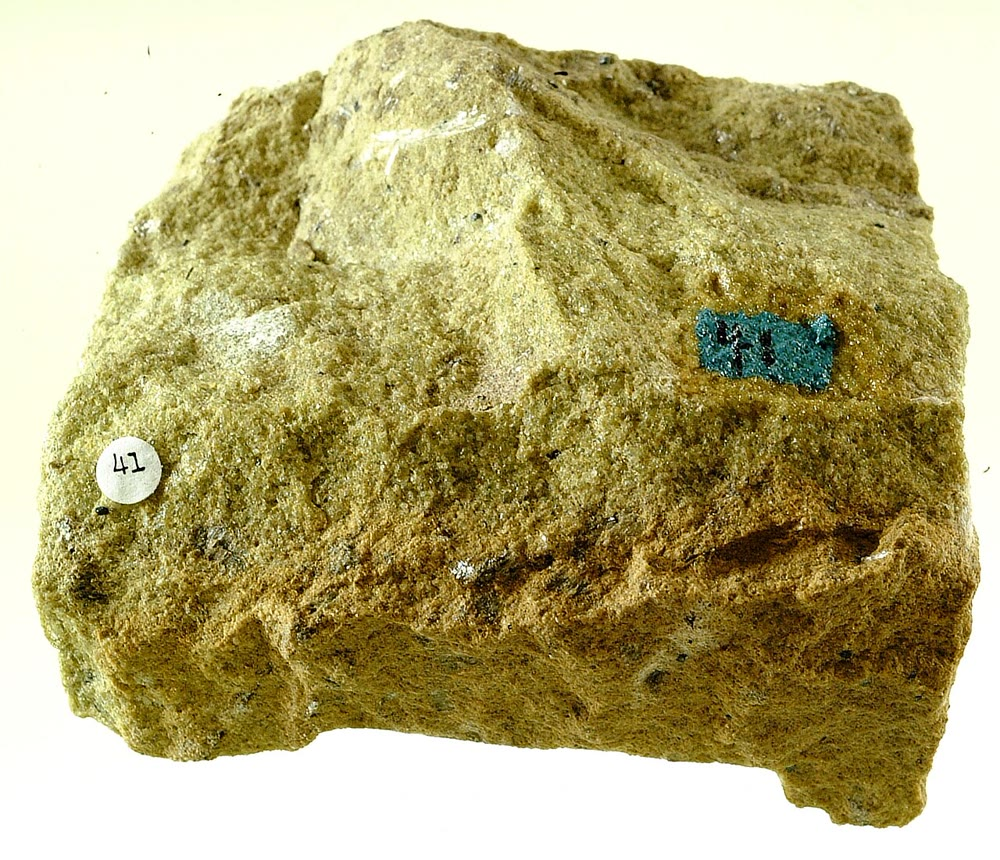
\includegraphics[width=\linewidth]{images/book4/b2-dunite.jpg}
\par\smallskip{\scriptsize Um \omterm{def:b2:mantle-melting:peridotites}{dunito}, quase inteiramente de olivina, com pequenos grãos negros
de cromita; a amostra tem \qty{8.5}{cm} de largura (Mike Davis, CC0).}
\end{minipage}
\end{inthefield}
% ledger: casetta23:kimberlite, tulane:ocean-basins (Book 2), bgs:ultramafic

\section{Exercícios}

\begin{exercise}[$\star$]\label{exo:b2:mantle-melting:1}
Dê o nome de cada rocha a partir de suas proporções de olivina, ortopiroxênio e clinopiroxênio
(por cento): (a) 93, 5, 2; (b) 75, 25, 0; (c) 60, 27, 13; (d) 30, 45, 25. (e) Dê
o nome do manto superior modelo (57, 28, 13 e \qty{2}{\percent} de espinélio) depois de
renormalizar seus três silicatos a \qty{100}{\percent}.
\end{exercise}
% ledger: bgs:ultramafic, liang21:dmm-mode

\begin{exercise}[$\star$]\label{exo:b2:mantle-melting:2}
No diagrama diopsídio--anortita, um líquido com \qty{60}{\percent} de anortita
se resfria. (a) A que temperatura ele começa a cristalizar, e que mineral
se forma? (b) A que temperatura aparece o segundo mineral, e qual é então
a composição do líquido? (c) Qual é a composição do primeiro líquido quando
uma rocha com \qty{80}{\percent} de diopsídio e \qty{20}{\percent} de anortita é aquecida,
e a que temperatura ele aparece?
\end{exercise}
% ledger: bowen15:di-an

\begin{exercise}[$\star$]\label{exo:b2:mantle-melting:3}
(a) Calcule o gradiente adiabático $\alpha T/(\rho c_p)$ em kelvins por gigapascal
para $T_p = \qty{1350}{\celsius}$, $\alpha = \qty{4.0e-5}{K^{-1}}$, $\rho =
\qty{3300}{kg/m^3}$, $c_p = \qty{1000}{J/(kg.K)}$. (b) Quantos quilômetros de
manto correspondem a um gigapascal ($g = \qty{9.81}{m/s^2}$)? Converta o gradiente em kelvins
por quilômetro e compare com um gradiente geotérmico típico perto da superfície,
cerca de \qty{30}{K/km}.
\end{exercise}
% ledger: katz03:thermo, earle:settings (Book 2)

\begin{exercise}[$\star$]\label{exo:b2:mantle-melting:4}
(a) Calcule o solidus seco do \omterm{def:b2:mantle-melting:peridotites}{peridotito} a 0, 1, 2 e \qty{3}{GPa}. (b) De quantos
graus ele sobe por gigapascal perto de \qty{2}{GPa}? (c) Explique em uma
frase por que um manto a \qty{1400}{\celsius} a \qty{3}{GPa} é sólido, e o
mesmo manto levado a \qty{2}{GPa} sem trocar calor está parcialmente fundido.
\end{exercise}
% ledger: katz03:solidus

\begin{exercise}[$\star\star$]\label{exo:b2:mantle-melting:5}
Um líquido com \qty{70}{\percent} de diopsídio e \qty{30}{\percent} de anortita se resfria.
(a) Estime sua temperatura do liquidus interpolando entre o liquidus a
\qty{20}{\percent} de anortita (\qty{1350}{\celsius}) e a \qty{40}{\percent}
(\qty{1277.5}{\celsius}). (b) Que mineral cristaliza primeiro? (c) Que fração em massa
do sistema cristalizou quando o líquido atinge o eutético?
(d) Quais são as proporções de diopsídio e de anortita na rocha final?
\end{exercise}
% ledger: bowen15:di-an

\begin{exercise}[$\star\star$]\label{exo:b2:mantle-melting:6}
(a) Calcule a porcentagem em massa de \ce{SiO2} na forsterita \ce{Mg2SiO4} e na
enstatita \ce{MgSiO3} ($M_{\ce{MgO}} = \qty{40.30}{g/mol}$, $M_{\ce{SiO2}} =
\qty{60.08}{g/mol}$). (b) Bowen e Andersen encontraram para o líquido peritético
\qty{97.5}{\percent} de \ce{MgSiO3} e \qty{2.5}{\percent} de \ce{SiO2}: qual é seu
teor de sílica? (c) Use a regra da alavanca para calcular a fração em massa de forsterita
formada quando a enstatita funde no peritético, e compare com seus
\qty{5.5}{\percent}. (d) O que isso implica para o teor de sílica de um fundido de
\omterm{def:b2:mantle-melting:peridotites}{peridotito} comparado com o de seu ortopiroxênio?
\end{exercise}
% ledger: bowen14:mgo-sio2

\begin{exercise}[$\star\star$]\label{exo:b2:mantle-melting:7}
Com a adiabática $T = T_p + 20P$ e o solidus seco do texto, calcule a
pressão e a profundidade ($\qty{30.9}{km}$ por gigapascal) em que a fusão começa
para (a) $T_p = \qty{1300}{\celsius}$ e (b) $T_p = \qty{1450}{\celsius}$. (c) De
quantos quilômetros por \qty{10}{\celsius} o início se aprofunda perto de
$T_p = \qty{1300}{\celsius}$? Use a \cref{prop:b2:mantle-melting:onset}.
\end{exercise}
% ledger: katz03:solidus

\begin{exercise}[$\star\star$]\label{exo:b2:mantle-melting:8}
A \qty{2.0}{GPa}, suponha que a \omterm{def:b2:mantle-melting:fraction}{fração de fundido} cresce linearmente do solidus seco até
o liquidus do \omterm{def:b2:mantle-melting:peridotites}{lherzolito} $T_{\mathrm l} = 1475.0 + 80.0P - 3.2P^2$. Para $F = 0.10$:
(a) calcule a temperatura da rocha que funde; (b) calcule $(\partial
T/\partial P)_F$ e $(\partial T/\partial F)_P$; (c) calcule a produtividade com
$c_p = \qty{1000}{J/(kg.K)}$, $\alpha/\rho = \qty{1.21e-8}{m^3/(kg.K)}$ e
$\Delta S = \qty{300}{J/(kg.K)}$. (d) Qual seria ela sem calor latente?
\end{exercise}
% ledger: katz03:solidus, katz03:melting, katz03:thermo

\begin{exercise}[$\star\star$]\label{exo:b2:mantle-melting:9}
(a) De quanto 1, 5 e \qty{13}{\percent} de água dissolvida no fundido rebaixam
o solidus? (b) Qual é o solidus saturado em água a \qty{1}{GPa}? (c) Um manto
contém \qty{125}{ppm} de água em massa, e o coeficiente de partição da água entre
minerais e fundido é 0.01. No início da fusão, o fundido contém $X =
X_{\text{total}}/D$: calcule-o e o rebaixamento do solidus que ele causa.
\end{exercise}
% ledger: katz03:water

\begin{exercise}[$\star\star\star$]\label{exo:b2:mantle-melting:10}
(a) Na \cref{prop:b2:mantle-melting:triangle}, verifique que o manto que entra pela
base do triângulo a cada ano é igual ao manto que sai por seus lados. Por que
os lados devem estar a \ang{45} para um manto que sobe a $U$ e sai a $U$?
(b) Mostre que, com produtividade constante $\Pi$ por gigapascal, $h_c = \Pi\,\rho
g\,z_0^2/2$ (com $P_0 = \rho g z_0$), de modo que a crosta cresce com o quadrado da
profundidade do início. (c) Uma dorsal se abre a uma velocidade total de \qty{50}{mm/yr} e
produz \qty{7.1}{km} de crosta: que volume de crosta cada quilômetro de dorsal
produz por ano, e que volume de manto ele funde se a \omterm{def:b2:mantle-melting:fraction}{fração de fundido} média for de
\qty{12}{\percent}?
\end{exercise}

\begin{exercise}[$\star\star\star$]\label{exo:b2:mantle-melting:11}
No sistema ternário da figura esquemática, o líquido $X$ tem
\qty{60}{\percent} de A, \qty{20}{\percent} de B e \qty{20}{\percent} de C; o
eutético binário $e_{AB}$ está em A 40, B 60 (por cento), e o \omterm{def:b2:mantle-melting:ternary}{eutético ternário} E em
A 25, B 30, C 45. (a) Escreva a composição do líquido quando uma fração em massa $t$
de A puro cristalizou, e mostre que a razão entre B e C permanece igual a 1. (b) A
cotética de $e_{AB}$ a E é a linha dos pontos $e_{AB} + s(E - e_{AB})$: encontre
onde o líquido a encontra, e a fração de A cristalizada até então. (c) Quando
o líquido atinge E, que fração do sistema ainda está líquida? (C não entra em nenhum
cristal antes de E.) (d) Quanto de A e quanto de B cristalizaram até então?
\end{exercise}

\begin{exercise}[$\star\star\star$]\label{exo:b2:mantle-melting:12}
O teor de água de um fundido saturado é $X_{\mathrm{sat}} = 12P^{0.6} + P$
(por cento, $P$ em gigapascals). (a) Calcule-o a 1 e a \qty{2}{GPa}, o rebaixamento
do solidus que ele produz, e o solidus saturado em água nas duas pressões. (b) Por que
o solidus saturado quase não muda entre 1 e \qty{2}{GPa}, enquanto o seco
sobe mais de \qty{100}{\celsius}? (c) Em uma cunha mantélica a \qty{2}{GPa} e
\qty{1100}{\celsius}, quanta água o fundido deve conter para que a rocha funda?
\end{exercise}
% ledger: katz03:water, katz03:solidus

\section{Problema: sob a dorsal}

\begin{problem}[{Problema de fim de semana --- da adiabática do manto à espessura da
crosta oceânica, e de volta à temperatura do manto}]
\label{pb:b2:mantle-melting:1}
O manto sobe sob uma dorsal ao longo da adiabática e funde. Dados: coeficiente de dilatação
térmica $\alpha = \qty{4.0e-5}{K^{-1}}$; densidade $\rho = \qty{3300}{kg/m^3}$;
calor específico $c_p = \qty{1000}{J/(kg.K)}$; entropia de fusão $\Delta S =
\qty{300}{J/(kg.K)}$; $g = \qty{9.81}{m/s^2}$; solidus seco $T_{\mathrm s} =
1085.7 + 132.9P - 5.1P^2$ e liquidus do \omterm{def:b2:mantle-melting:peridotites}{lherzolito} $T_{\mathrm l} = 1475.0 +
80.0P - 3.2P^2$ (\unit{\celsius}, $P$ em \unit{GPa}); produtividade média do
modelo de fusão ajustado, $\Pi = \qty{9}{\percent}$ por gigapascal; coeficiente de reação
do clinopiroxênio perto da superfície 0.50; crosta observada \qty[uncertainty-mode=separate]{7.1 \pm 0.8}{km}
nas dorsais normais e \qty{20}{km} sobre o centro da pluma da Islândia. Tome o manto
e a crosta com a mesma densidade.

\noindent\textbf{Parte I --- Onde a fusão começa.}
\begin{enumerate}
\item Converta $T_p = \qty{1350}{\celsius}$ em kelvins.
\item Calcule o gradiente adiabático $\alpha T_p/(\rho c_p)$ em kelvins por
gigapascal, e arredonde-o para a dezena mais próxima.
\item Quantos quilômetros de manto correspondem a um gigapascal? Dê o gradiente em
kelvins por quilômetro.
\item Com a adiabática $T = 1350 + 20P$, escreva a equação do segundo grau para a pressão de início
$P_0$ e resolva-a.
\item Dê a profundidade e a temperatura em que a fusão começa.
\item Verifique que o solidus em $P_0$ dá a mesma temperatura.
\end{enumerate}

\noindent\textbf{Parte II --- Quanto fundido.}
\begin{enumerate}[resume]
\item A \qty{1.5}{GPa}, calcule o solidus, o liquidus do \omterm{def:b2:mantle-melting:peridotites}{lherzolito} e sua
diferença.
\item Com uma \omterm{def:b2:mantle-melting:fraction}{fração de fundido} que cresce linearmente entre eles, dê a temperatura da
rocha em $F = 0.10$, em graus Celsius e em kelvins.
\item Calcule ali $(\partial T/\partial P)_F$ e $(\partial T/\partial F)_P$.
\item Calcule a produtividade da \cref{prop:b2:mantle-melting:productivity}, em
por cento por gigapascal.
\item O modelo ajustado dá $\Pi = \qty{9}{\percent}$ por gigapascal em média.
Por que é menor? Com $\Pi$, qual é a \omterm{def:b2:mantle-melting:fraction}{fração de fundido} $F_{\max}$ atingida na
superfície?
\item O manto modelo contém \qty{13}{\percent} de clinopiroxênio. Em que \omterm{def:b2:mantle-melting:fraction}{fração de fundido}
ele se esgota perto da superfície? O resíduo sob o eixo é um
\omterm{def:b2:mantle-melting:peridotites}{lherzolito} ou um \omterm{def:b2:mantle-melting:peridotites}{harzburgito}?
\end{enumerate}

\noindent\textbf{Parte III --- A crosta.}
\begin{enumerate}[resume]
\item Use a \cref{prop:b2:mantle-melting:triangle} com $H = z_0$ para calcular a
espessura da crosta.
\item Qual é a \omterm{def:b2:mantle-melting:fraction}{fração de fundido} média do fundido agregado?
\item Compare com a espessura observada.
\item O modelo completo da figura dá \qty{9.0}{km}. Por que é mais delgado que
sua estimativa?
\item Mostre que $h_c = k P_0^2$ e calcule $k$ em quilômetros por gigapascal
ao quadrado.
\end{enumerate}

\noindent\textbf{Parte IV --- A temperatura do manto.}
\begin{enumerate}[resume]
\item Calcule a pressão de início $P_0$ que produz \qty{7.1}{km} de crosta.
\item Dê a profundidade correspondente do início.
\item Com a adiabática $T = T_p + 20P$, calcule a temperatura potencial que
coloca o início nessa pressão.
\item Refaça o cálculo para 6.3 e \qty{7.9}{km}: que intervalo de $T_p$ a
dispersão da crosta permite?
\item A crosta tem \qty{20}{km} de espessura sobre o centro da pluma da Islândia. Calcule
ali a temperatura potencial, e seu excesso sobre a da questão~20.
\item As lavas das ilhas oceânicas sugerem plumas 200 a \qty{300}{\celsius} mais quentes que
o manto ambiente. Sugira por que a crosta dá um excesso menor.
\item Em quantos por cento a crosta se espessa para um manto \qty{10}{\celsius}
mais quente, perto da dorsal normal?
\item As dorsais muito lentas produzem crosta mais delgada. Explique por quê com o triângulo.
\item Indique a \omterm{def:b2:mantle-melting:tp}{temperatura potencial do manto} sob uma dorsal normal que
a espessura da crosta dá, o número-chave deste problema, e compare-a
com os \qty{1350}{\celsius} da física mineral e com o intervalo de 1280 a
\qty{1400}{\celsius} das lavas.
\end{enumerate}
\end{problem}
% ledger: katz03:solidus, katz03:melting, katz03:thermo, white:crust (Book 3), herzberg:tp (Book 3), katsura:adiabat (Book 3)
